\section*{Mini Machine Problem 1 }

\textbf{Answers} 


\begin{enumerate}
\item[1.] Load the data \textbf{carsmall} in Matlab using the following code.
\begin{lstlisting}
load carsmall
X = [MPG,Acceleration,Displacement,Weight,Horsepower];
varNames = {'MPG'; 'Acceleration'; 'Displacement'; 'Weight'; 'Horsepower'};
\end{lstlisting}
\item[2.] (Comet graph is an animated graph. To trace the data points on the screen for the \texttt{Displacement} attribute, we use the following code to visualize the \texttt{Displacement} attribute. Show the \textbf{final comet graph} in the PDF file you will submit by running the following code on Matlab.
\begin{lstlisting}
comet(Displacement)
xlabel('Index of Car')
ylabel('Displacement')
\end{lstlisting}

  \begin{figure}[h]
  \centering
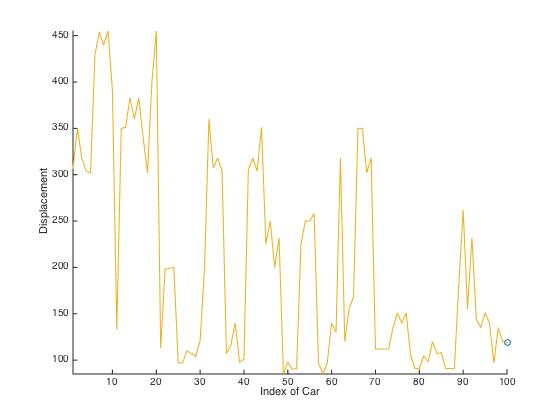
\includegraphics[width=10cm, height=10cm]{mp12}
  \end{figure}
  

\item[3.] (5') Drawing boxlpot is a popular way to visualize a distribution. The two whiskers show the Min observation and the Max observation. The central line shows the median. The edges of the box are the first quantile and the third quantile. 
\begin{itemize}
\item[a.] (1') Run the following code on your Matlab to draw a boxplot for the \texttt{Acceleration} attribute. Show the \textbf{boxplot}  in the PDF file you will submit.
\begin{lstlisting}
boxplot(Acceleration)
ylabel('Acceleration')
\end{lstlisting}
  \begin{figure}[h]
  \centering
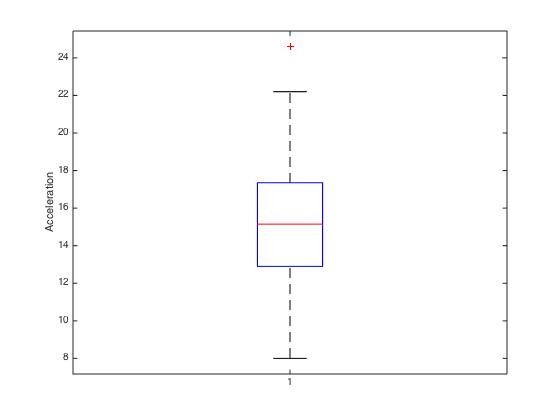
\includegraphics[width=10cm, height=10cm]{mp13a}
  \end{figure}
  

\item[b.] 

\begin{lstlisting}
boxplot(Acceleration,Cylinders)
xlabel('Cylinders')
ylabel('Acceleration')
\end{lstlisting}

  \begin{figure}[H]
  \centering
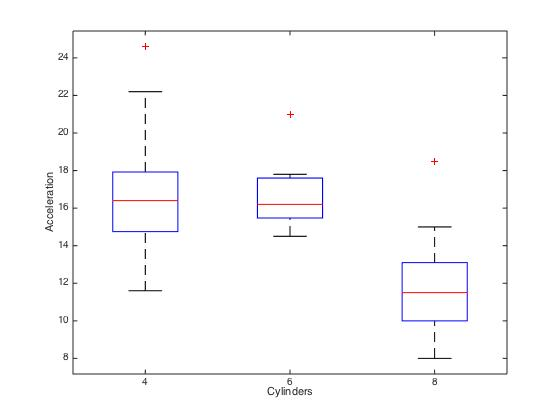
\includegraphics[width=10cm, height=10cm]{mp13b}
  \end{figure}
  

\item[4.] (4') 3-D scatter plots are popularly used to visualize 3 attributes at the same time. 
\begin{itemize}
\item[a.] (2') Run the following code to draw a 3-D scatter plot. Show the \textbf{3-D plot} in the PDF file you will submit. 
\begin{lstlisting}
scatter3(Displacement,Cylinders,Horsepower,'filled','r')
xlabel('Displacement')
ylabel('Cylinders')
zlabel('Horsepower')

\end{lstlisting}
  \begin{figure}[H]
  \centering
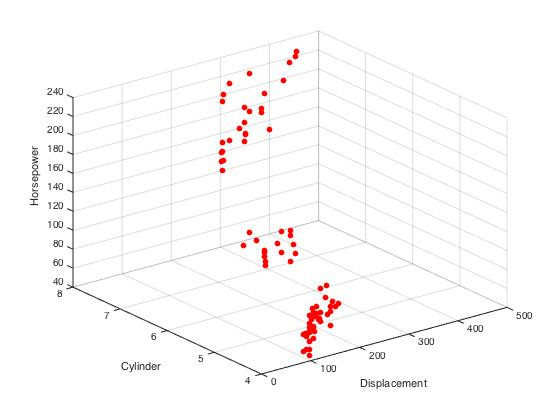
\includegraphics[width=10cm, height=10cm]{mp14}
  \end{figure}
  


\item[b.] 
Horsepower and displacement a pair of positively correlated attributes.
Displacement is the total volume of all the cylindets in an engine. Larger engines tend to produce more power, more turque. 
\end{itemize}

\item[5.] (4') Interactive star plots are used to show the values of attributes for each observation. In each star (observation), the spoke length is proportional to the value of that attribute for that observation.
\begin{itemize}
\item[a.] (2') Run the following code. Show the \textbf{graph} in PDF file you will submit.
\begin{lstlisting}
h = glyphplot(X(1:9,:), 'glyph','star', 'varLabels',varNames,...
'obslabels',Model(1:9,:));
set(h(:,3),'FontSize',8);
\end{lstlisting}

  \begin{figure}[H]
  \centering
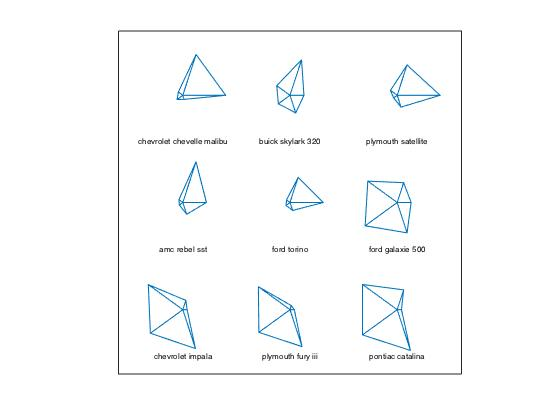
\includegraphics[width=10cm, height=10cm]{mp15}
  \end{figure}
  

\item[b.] 
Observation: Chevrolet chevelle malibu

MPG: 18

Acceleration: 12

Displacement: 307

Weight: 3504

Horsepower: 130

\end{itemize}

\end{enumerate}